\chapter{Expérimentations et résultats}

\section*{Introduction}
En général, il y a deux catégories de problèmes d'optimisation, les fonctions de test et les problèmes du monde réel. Les fonctions de test sont des problèmes artificiels qui peuvent être utilisés pour l'évaluation d'un algorithme dans différentes situations avec plusieurs niveaux de difficulté.

Les problèmes du monde réel touchent à différents domaines tels la physique, la chimie, l'ingénierie et les mathématiques. Ces problèmes sont plus difficiles à manipuler que les fonctions de test artificielles, mais ils se ramèment toujours à une ou à plusieurs d'entre elles.

Après l'implémentation de CBSO, nous pouvons donner les fonctions de test utilisées ainsi que les paramètres de l'algorithme. Ensuite, nous présentons les résultats de nos expérimentations qui sont une phase très importante pour l'évaluation de notre travail. Enfin, nous faisons une étude comparative entre CBSO et d'autres algorithmes d'optimisation continue en vue d'examiner les performances de CBSO et sa capacité de converger vers l'optimum global face aux fonctions multimodales.

\section{Fonctions de test}
Nous avons mené nos expérimentations sur des benchmarks publics utilisés par des méthodes avec lesquelles nous envisageons une comparaison. Ces benchmarks contiennent des fonctions de test de plusieurs types dont les optimums globaux sont connus.

Les fonctions multi-modales avec plusieurs optimums locaux sont parmi les classes de problèmes les plus difficiles, tandis que les fonctions à surfaces plates posent une difficulté à l'algorithme parce qu'elles ne donnent pas d'information pour le diriger vers l'optimum. 

\vspace{2em}La liste des fonctions de test que nous avons utilisées est la suivante\cite{Momin_Yang_2013}.
\begin{itemize}
	\item
	Diagonal Plane ($DP$)\\$$DP(\overrightarrow{x})=\frac{1}{n}\sum_{i=1}^{n} x_i$$
	
	\begin{itemize}[label={$\circ$}]
		\item $n=$10, 
		\item $\overrightarrow{x} \in [0.5,1.5]^n$,
		\item $h_0=10^{-22}$,
		\item $h_k=7*10^{-21}$,
		\item optimum global DP(0.5,...,0.5)=0.5,
		\item continue, non-séparable et uni-modale.
	\end{itemize}
	
	\bigskip
	\bigskip
	\item
	Sphere ($SP$)\\$$SP(\overrightarrow{x})=\sum_{i=1}^{n} x_i^2$$

	\begin{itemize}[label={$\circ$}]  
		\item $n=$10, 
		\item $\overrightarrow{x} \in [-3,7]^n$,
		\item $h_0=10^{-5}$,
		\item $h_k=10^{-1}$,
		\item optimum global SP(0,...,0)=0,
		\item continue, séparable et multi-modale.
	\end{itemize}
	
	\bigskip
	\bigskip
	\item
	$B_2$\\$$B_2(\overrightarrow{x})=(x_1^2+2x_2^2-0.3\cos(3\pi x_1)-0.4\cos(4\pi x_2)+0.7)$$

	\begin{itemize}[label={$\circ$}]
		\item $n=$2,
		\item $\overrightarrow{x} \in [-100,100]^n$,
		\item $h_0=3*10^{-3}$,
		\item $h_k=2$,
		\item optimum global B$_2$(0,0)=0,
		\item continue, non-séparable et multi-modale.
	\end{itemize}
	
	\bigskip
	\bigskip
	\item
	Branin RCOS 
	($RC$)\\$$RC(\overrightarrow{x})=\left(x_2-\left(\frac{5}{(4\pi^2)}\right)x_1^2+\left(\frac{5}{\pi}\right)x_1-6\right)^2+10\left(1-\left(\frac{1}{8\pi}\right)\right)\cos(x_1) +10$$

	\bigskip

	\begin{itemize}[label={$\circ$}]
		\item $n=$2, 
		\item $\overrightarrow{x} \in [-5,15]^n$,
		\item $h_0=6*10^{-4}$,
		\item $h_k=8*10^{-1}$,
		\item optimums globaux RC(-$\pi$,12.275)=0.39, RC($\pi$,2.275)=0.39, RC(9.42478,2.475)=0.39,
		\item continue, non-séparable et multi-modale.
	\end{itemize}
	
	\bigskip
	\bigskip
	\item
	Easom ($ES$)\\$$ES(\overrightarrow{x})= -\cos (x_1)\cos (x_2) \exp (-((x_1-\pi )^2+(x_2-\pi)^2))$$

	\begin{itemize}[label={$\circ$}]
		\item $n=$2,
		\item $\overrightarrow{x} \in [-100,100]^n$,
		\item $h_0=8*10^{-4}$,
		\item $h_k=2$,
		\item optimum global ES($\pi$,$\pi$)=-1,
		\item continue, séparable et multi-modale.
	\end{itemize}
	
	\bigskip
	\bigskip
	\item
	De Joung ($DJ$)\\$$DJ(\overrightarrow{x})= x_1^2+x_2^2+x_3^2$$
	
	\begin{itemize}[label={$\circ$}]
		\item $n=$3, 
		\item $\overrightarrow{x} \in [-5.12,5.12]^n$,
		\item $h_0=3*10^{-4}$,
		\item $h_k=4*10^{-1}$,
		\item optimum global DJ(0,0,0)=0,
		\item continue, séparable et multi-modale.
	\end{itemize}
	
	\bigskip
	\bigskip
		\bigskip
	\bigskip
	\item
	Rosenbrock2 ($R_2$)\\$$R_n(\overrightarrow{x})= \sum_{i=1}^{n-1} [100(x_i^2-x_{i+1})^2+(x_i -1)^2]$$
	\begin{itemize}[label={$\circ$}]
		\item $n=$2, 
		\item $\overrightarrow{x} \in [-5,10]^n$,
		\item $h_0=10^{-2}$,
		\item $h_k=1$,
		\item optimum global R$_n$(1,...,1)=0,
		\item continue, non-séparable et uni-modale.
	\end{itemize}
	\bigskip
	\item Zakharov2 ($Z_2$)
	
	\bigskip
	
	$$Z_n(\overrightarrow{x})= \left(\sum_{i=1}^{n}x_i^2\right) + \left(\sum_{i=1}^{n} 0.5ix_i\right)^2 + \left(\sum_{i=1}^{n} 0.5ix_i\right)^4$$
	
	\bigskip
	
	\begin{itemize}[label={$\circ$}]
		\item $n=$2,
		\item $\overrightarrow{x} \in [-5,10]^n$,
		\item $h_0=10^{-2}$,
		\item $h_k=2*10^{-1}$,
		\item optimum global Z$_n$(0,...,0)=0,
		\item continue, non-séparable et multi-modale.
	\end{itemize}
	
	\bigskip
	\bigskip
	\item Zakharov5 ($Z_5$)\\$$Z_n(\overrightarrow{x})= \left(\sum_{i=1}^{n}x_i^2\right) + \left(\sum_{i=1}^{n} 0.5ix_i\right)^2 + \left(\sum_{i=1}^{n} 0.5ix_i\right)^4$$
	
	\begin{itemize}[label={$\circ$}]
		\item $n=$5,
		\item $\overrightarrow{x} \in [-5,10]^n$,
		\item $h_0=2*10^{-3}$,
		\item $h_k=2*10^{-1}$,
		\item optimum global Z$_n$(0,...,0)=0,
		\item continue, non-séparable et multi-modale.
	\end{itemize}
	\bigskip
	\bigskip
	\item
	Hartmann$_3$ ($H_{3,4}$)\\$$H_{3,4}(\overrightarrow{x})= -\sum_{i=1}^{4} c_i \exp[-\sum_{j=1}^{3}a_{ij}(x_j-p_{ij})^2]$$
	
	\begin{itemize}[label={$\circ$}]
		\item $n=$3, 
		\item $\overrightarrow{x} \in [0,1]^n$,
		\item $h_0=6*10^{-5}$,
		\item $h_k=8*10^{-2}$,
		\item optimum global H$_{3,4}$(0.1140,0.556,0.852)=-3.86,
		\item continue, non-séparable et multi-modale (4 optimums locaux).
	\end{itemize}
	
	\bigskip
	
	\begin{table}[H]\centering
		\begin{tabular}{ccc|c|ccc}
			\toprule \textbf{} & \textbf{$a_{ij}$} & \textbf{} & \textbf{$c_i$} & \textbf{} & \textbf{$p_{ij}$}  \\    \midrule
			3.0 & 10. & 30. & 1.0 &0.3689 &0.1170 &0.2673   \\  
			0.1 & 10. & 35. & 1.2 &0.4699 &0.4387 &0.7470   \\ 
			3.0 & 10. & 30. & 3.0 &0.1091 &0.8732 &0.5547   \\
			0.1 & 10. & 35. & 3.2 &0.0381 &0.5743 &0.8828   \\ 
			\bottomrule	
		\end{tabular}
	\end{table}
	\bigskip
	\bigskip
	\item
	Hartmann$_6$ ($H_{6,4}$)\\$$H_{6,4}(\overrightarrow{x})= -\sum_{i=1}^{4} c_i \exp[-\sum_{j=1}^{6}a_{ij}(x_j-p_{ij})^2]$$

	\begin{itemize}[label={$\circ$}]
		\item $n=$6, 
		\item $\overrightarrow{x} \in [0,1]^n$,
		\item $h_0=10^{-3}$,
		\item $h_k=2*10^{-2}$,
		\item optimum global H$_{6,4}$(0.2016,0.1500,0.4768,0.2753,0.3116,0.6573)=-3.32,
		\item continue, non-séparable et multi-modale (4 optimums locaux).
	\end{itemize}

	\bigskip

	\begin{table}[H]\centering
		\begin{tabular}{cccccc|c|cccccc}
			\toprule \textbf{} & \textbf{} & \textbf{$a_{ij}$} & \textbf{} & \textbf{} & \textbf{} & \textbf{$c_i$} & \textbf{} & \textbf{} & \textbf{} & \textbf{$p_{ij}$} & \textbf{} & \textbf{}  \\    \midrule
			10. & 3. & 17. & 3.5 & 1.7 & 8. & 1.0 & 0.1312 & 0.1696 & 0.5569 & 0.0124 & 0.8283 & 0.5886 \\  
			0.05 & 10. & 17. & 0.1 & 8.0 & 14.0 & 1.2 & 0.2329 & 0.4135 & 0.8307 &0.3736 & 0.1004 & 0.9991  \\ 
			3.0 & 3.5 & 1.7 & 10.0 & 17.0 & 8.0 & 3.0 & 0.2348 & 0.1451 & 0.3522 & 0.2883 & 0.3047 & 0.6650  \\
			17.0 & 8.0 & 0.05 & 10.0 & 0.1 & 14.0 & 3.2 & 0.4047 & 0.8828 & 0.8732 & 0.5743 &0.1091 &0.0381  \\ 
			\bottomrule	
		\end{tabular}
	\end{table}
	\vspace{5em}
	\item Shekel$_5$ ($S_{4,5}$)\\$$S_{4,5}(\overrightarrow{x})= -\sum_{i=1}^{5} [(\overrightarrow{x}-a_i)^T(\overrightarrow{x}-a_i)+c_i]^{-1}$$

	\begin{itemize}[label={$\circ$}]
		\item $n=$4, 
		\item $\overrightarrow{x} \in [0,10]^n$,
		\item $h_0=6*10^{-5}$,
		\item $h_k=2*10^{-2}$,
		\item optimum global S$_{4,5}$(4,4,4,4)=-10.14,
		\item continue, non-séparable et multi-modale (5 optimums locaux).
	\end{itemize}

	\bigskip

	\begin{table}[H]\centering
		\begin{tabular}{cccc|c}
			\toprule \textbf{} & \textbf{$a_{ij}$} & \textbf{} & \textbf{} & \textbf{$c_i$}\\    \midrule
			4 & 4 & 4 & 4 & 0.1    \\  
			1 & 1 & 1 & 1 & 0.2   \\ 
			8 & 8 & 8 & 8 & 0.2  \\
			6 & 6 & 6 & 6 & 0.4   \\ 
			3 & 7 & 3 & 7 & 0.4 \\ 
			\bottomrule	
		\end{tabular}
	\end{table}

	\bigskip

	\item Shekel$_7$ ($S_{4,7}$)\\$$S_{4,7}(\overrightarrow{x})= -\sum_{i=1}^{7} [(\overrightarrow{x}-a_i)^T(\overrightarrow{x}-a_i)+c_i]^{-1}$$

	\begin{itemize}[label={$\circ$}]
		\item $n=$4, 
		\item $\overrightarrow{x} \in [0,10]^n$,
		\item $h_0=6*10^{-5}$,
		\item $h_k=2*10^{-2}$,
		\item optimum global S$_{4,7}$(4,4,4,4)=-10.39,
		\item continue, non-séparable et multi-modale (7 optimums locaux).
	\end{itemize}

	\bigskip

	\begin{table}[H]\centering
		\begin{tabular}{cccc|c}
			\toprule \textbf{} & \textbf{$a_{ij}$} & \textbf{} & \textbf{} & \textbf{$c_i$} \\    \midrule
			4 & 4 & 4 & 4 & 0.1    \\  
			1 & 1 & 1 & 1 & 0.2   \\ 
			8 & 8 & 8 & 8 & 0.2  \\
			6 & 6 & 6 & 6 & 0.4   \\ 
			3 & 7 & 3 & 7 & 0.4 \\ 
			2 & 9 & 2 & 9 & 0.6   \\ 
			5 & 5 & 3 & 3 & 0.3 \\ 
			\bottomrule	
		\end{tabular}
	\end{table}
	
	\bigskip
	\bigskip
	\bigskip
	\item Shekel$_{10}$ ($S_{4,10}$)
	
	\bigskip
	$$S_{4,10}(\overrightarrow{x})= -\sum_{i=1}^{10} [(\overrightarrow{x}-a_i)^T(\overrightarrow{x}-a_i)+c_i]^{-1}$$
	\begin{itemize}[label={$\circ$}]
		\item $n=$4, 
		\item $\overrightarrow{x} \in [0,10]^n$,
		\item $h_0=6*10^{-5}$,
		\item $h_k=2*10^{-2}$,
		\item optimum global S$_{4,10}$(4,4,4,4)=-10.53,
		\item continue, non-séparable et multi-modale (10 optimums locaux).
	\end{itemize}

	\bigskip
	\bigskip
	
	\begin{table}[H]\centering
		\begin{tabular}{cccc|c}
			\toprule \textbf{} & \textbf{$a_{ij}$} & \textbf{} & \textbf{} & \textbf{$c_i$} \\    \midrule
			4 & 4 & 4 & 4 & 0.1  \\  
			1 & 1 & 1 & 1 & 0.2  \\ 
			8 & 8 & 8 & 8 & 0.2  \\
			6 & 6 & 6 & 6 & 0.4  \\ 
			3 & 7 & 3 & 7 & 0.4  \\ 
			2 & 9 & 2 & 9 & 0.6  \\ 
			5 & 5 & 3 & 3 & 0.3  \\ 
			8 & 1 & 8 & 1 & 0.7  \\ 
			6 & 2 & 6 & 2 & 0.5  \\ 
			7 & 3.6 & 7 & 3.6 & 0.5  \\ 
			\bottomrule	
		\end{tabular}
	\end{table}
	
\end{itemize}

\vspace{1.5em}

Comme nous l'avons expliqué, la représentation graphique d'une fonction est impossible si elle comporte plus de deux variables. Nous donnons ici la représentation de quelques fonctions à deux variables :

\begin{figure}[H]
	\centering
	\begin{subfigure}{0.3\textwidth}
		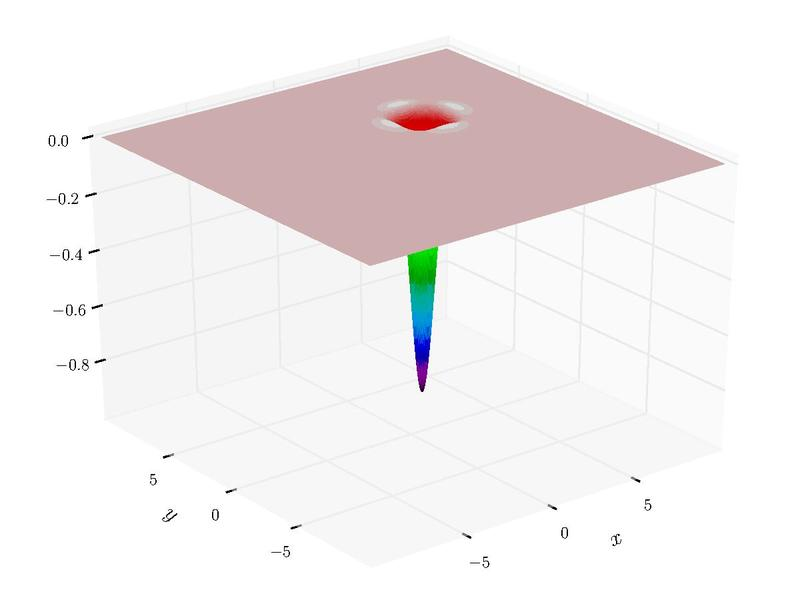
\includegraphics[width=\textwidth]{ES}
		\caption{Easom}
	\end{subfigure}
	\begin{subfigure}{0.3\textwidth}
		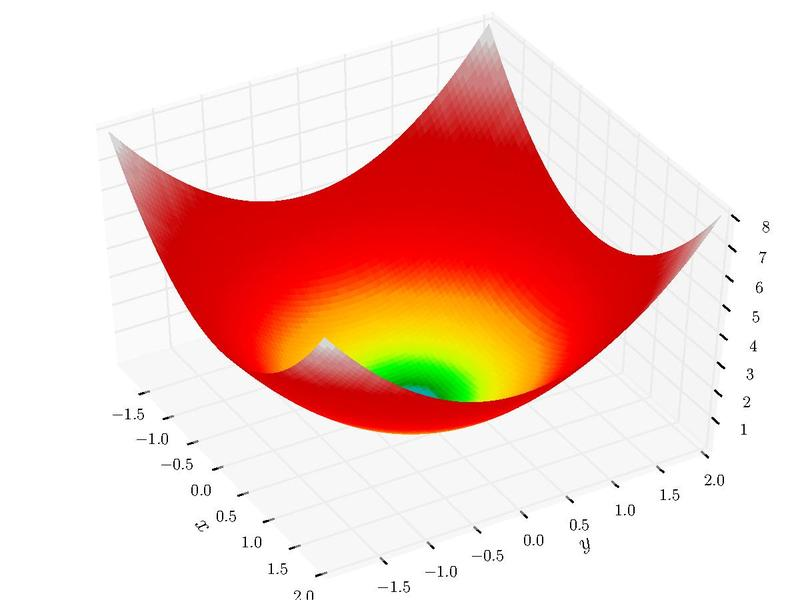
\includegraphics[width=\textwidth]{SP}
		\caption{Sphere}
	\end{subfigure}
	\begin{subfigure}{0.3\textwidth}
		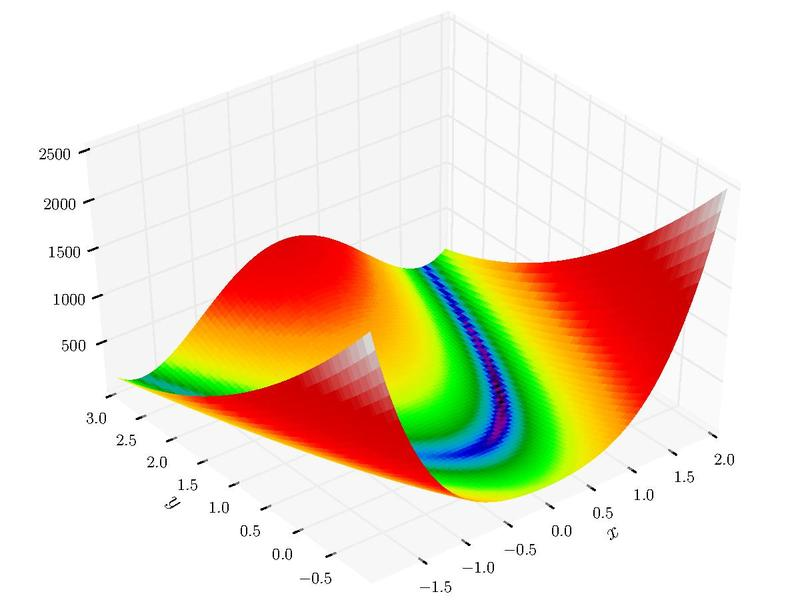
\includegraphics[width=\textwidth]{R}
		\caption{RosenBrock2}
	\end{subfigure}
	\caption{Représentation graphique de quelques fonctions de test à deux variables}
\end{figure}

\section{Paramètres de CBSO}
Chaque algorithme d'optimisation est caractérisé par un certain nombre de paramètres qui le définissent et le guident dans le processus de recherche de solution. La liste des paramètres que nous avons utilisés dans CBSO est la suivante.

\begin{table}[H]\centering
	\begin{tabular}{cp{0.5\textwidth}c}
		\toprule \textbf{Paramètre} & \textbf{Signification} & \textbf{Valeur}  \\    \midrule
		$m$ & Nombre d'abeilles. & $4$   \\   
		$k$ & Nombre de voisins. & $5$  \\   
		$SearchIter$ & Nombre d'itérations d'une recherche locale. & $10$ \\   
		$\xi$ & Vitesse de convergence de la solution noyau. & $0.0001$  \\     \addlinespace 
		$Stag$ & Nombre toléré d'itérations avant de détecter la stagnation. & $5000$ \\ \addlinespace 
		$MaxChances$ & Nombre maximum de chances pour améliorer le sommet de référence. & $3$   \\ \addlinespace 
		$1/Flip$ & Pourcentage de variables à remplacer dans le $SRef$. & 1/2   \\ \addlinespace 
		$MaxIter$ & Nombre maximum des itérations pour trouver la solution. & $50000$  \\ \addlinespace 
		$\epsilon$ & Précision voulue: différence tolérée entre l'évaluation de la solution et l'optimum global. & $10^{-4}$   \\		
		\bottomrule	
	\end{tabular}
	\caption{Paramètres de CBSO\label{key}}
\end{table}

\vspace{-1.2em}

\section{Analyse de CBSO}

\vspace{-0.5em}

Comme nous l'avons précisé, l'utilisateur visualise, à partir de l'interface graphique, le graphe représentant l'évolution de l'évaluation du sommet de référence au cours des itérations. La figure suivante montre ce graphe pour la fonction \emph{De Joung}.\bigskip

\begin{figure}[H]
	\centering
	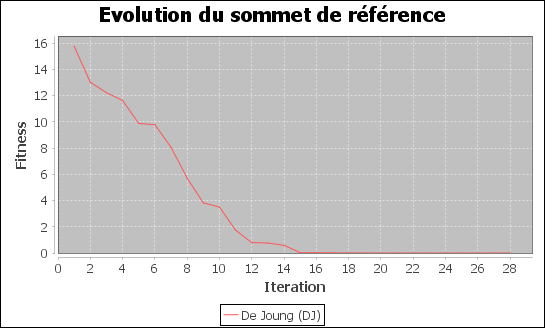
\includegraphics[width=0.65\textwidth,keepaspectratio]{DeJoung}
	\caption{Evolution de $SRef$ pour la fonction $De~Joung$}
\end{figure}

Nous remarquons que CBSO converge bien vers l'optimum. En commençant à partir d'une solution aléatoire qui a une grande évaluation, l'algorithme se rapproche petit à petit de la solution qui a la plus petite évaluation.

Lorsqu'il s'agit des fonctions multi-modales, nous remarquons des sauts dans l'évaluation du sommet de référence dans le graphe. Ces pics indiquent les moments de diversification où l'algorithme décide à régresser pour mieux avancer. Cela se traduit par un changement de la région à explorer de l'espace de recherche.

Nous donnons comme exemple la fonction multi-modale $Shekel_{4,10}$.\bigskip
\begin{figure}[H]
	\centering
	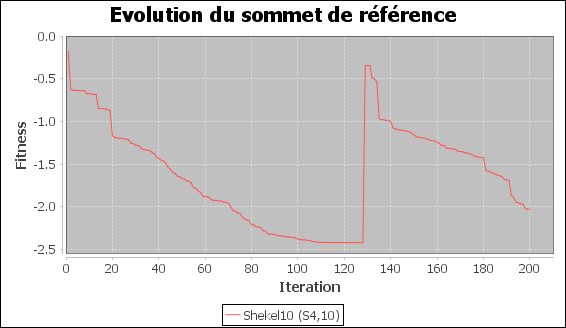
\includegraphics[width=0.65\textwidth,keepaspectratio]{Shekel}
	\caption{Evolution de $SRef$ pour la fonction $Shekel_{4,10}$}
\end{figure}

Pour simplifier, supposons que nous sommes face à une fonction à une seule variable. La figure suivante montre l'utilité de diversification en cas de stagnation dans un optimum local.

\begin{figure}[H]
	\centering
	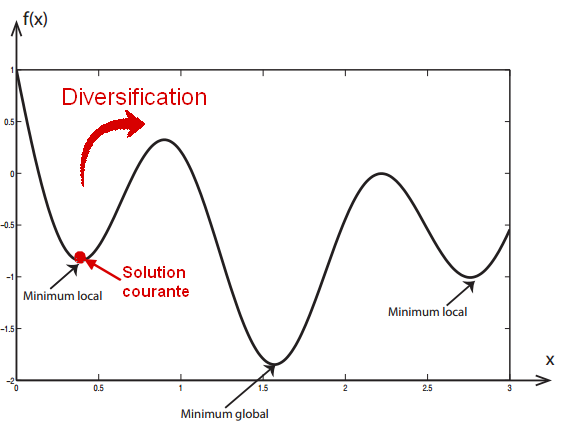
\includegraphics[width=0.70\textwidth,keepaspectratio]{diversification}
	\caption{Utilité de la diversification pour le changement de la zone de recherche}
\end{figure}

La diversification dans CBSO est faite lorsque le nombre de chances pour améliorer le sommet de référence devient nul, et cela par le choix de la meilleure solution en diversité à partir de la table $Danse$, c'est-à-dire la solution la plus éloignée des sommets de référence précédents. Dans le cas échéant, la diversification est faite en choisissant un sommet de référence aléatoire et cela lorsque toutes les solutions de la table $Danse$ sont taboues. 

Parmi les tâches les plus difficiles d'un algorithme d'optimisation, il y a celle de pouvoir diversifier au bon moment et vers la bonne région de l'espace de recherche, car une diversification aléatoire peut nous éloigner de l'optimum global et nous mener vers un autre optimum local.

\section{Mesure de comparaison entre les algorithmes}
\begin{spacing}{1.5}
	Selon les auteurs des algorithmes de l'optimisation continue, la comparaison entre ces algorithmes n'est pas basée sur le temps d'exécution mais sur \textbf{le nombre des évaluations de la fonction objectif} nécessaire pour atteindre la qualité de solution voulue \cite{SOCHA_DORIGO_2006}.
\end{spacing}

\bigskip

D'après eux, cette méthode présente quelques avantages:

\bigskip

\begin{itemize}
	\item résolution du problème des algorithmes implémentés en utilisant
	différents langages de programmation,
	\item insensibilité aux compétences du programmeur en termes
	d'optimisation du code,
	\item insensibilité à la performance du compilateur utilisé,
	\item facilité de comparaison des résultats obtenus par
	différentes machines.
\end{itemize}

Nous remarquons que cette méthode ne prend pas en considération la complexité de l'algorithme qui pourtant s'avère primordiale pour indiquer sa rapidité. En effet, la bonne mesure d'évaluation doit tenir compte de l'effectivité et de l'efficience de la méthode et exprimer le rapport entre ces deux critères.

Nous avons adopté cette méthode pour comparer CBSO aux autres algorithmes d'optimisation continue, mais nous présentons quand même le temps d'exécution de CBSO pour chaque fonction de test afin de permettre aux chercheurs de comparer leurs résultats avec les nôtres.\\

\begin{table}[H]\centering
	\begin{tabular}{cccccccccccccc}
		\toprule \textbf{DP} & \textbf{SP} & \textbf{B$_2$} & \textbf{RC} & \textbf{ES} & \textbf{DJ} & \textbf{R$_2$} & \textbf{H$_{3,4}$} & \textbf{H$_{6,4}$} & \textbf{S$_{4,5}$} & \textbf{S$_{4,7}$} & \textbf{S$_{4,10}$} & \textbf{Z$_2$} & \textbf{Z$_5$} \\    \midrule
		205 & 19 & 1794 & 1 & 15 & 2 & 10 & 10 & 262 & 416 & 400 & 351 & 1  & 8 \\
		\bottomrule	
	\end{tabular}
	\caption{Temps d'exécution de CBSO pour les fonctions en $millisecondes$\label{exe_table}}
\end{table}

Malgré l'espace de recherche infini, nous remarquons que CBSO est très rapide bien que les méta-heuristiques sont en général un peu lentes.\\

Nous avons comparé CBSO avec plusieurs algorithmes d'optimisation continue:

\begin{itemize}
	\item ceux basés sur l'apprentissage des probabilités qui
	modélisent et échantillonnent explicitement des distributions des
	probabilités (CSA-ES, (1+1)ES, CMA-ES, IDEA et MBOA),
	\item ceux qui s'inspirent du comportement naturel des fourmis (ACO$_\mathbb{R}$, ACO$_\mathbb{R}$-PT, CACO et CIAC),
	\item ceux qui ont été initialement développés pour
	les problèmes combinatoires et qui ont été adaptés par la suite aux problèmes continus (CGA, ECTS, ESA, TS, CTS, INTEROPT, CRTS$_{min}$ et CRTS$_{ave}$).
\end{itemize}

\begin{spacing}{1.5}
	Pour assurer une comparaison juste, nous répliquons le même environnement de test utilisé par les autres algorithmes, en particulier le domaine de définition des fonctions et la précision souhaitée.
\end{spacing}
\section{Évaluation de CBSO}
Pour une meilleure précision, nous avons mené $1000$ exécutions indépendantes pour chaque fonction de test et nous avons considéré la moyenne du nombre des évaluations de chaque fonction.
 
Le meilleur algorithme d'optimisation continue est celui qui présente le plus petit nombre d'évaluations des fonctions. Les résultats d'un tel algorithme sont donnés en gras dans les tableaux suivants.

Le taux des exécutions réussies (où l'algorithme n'est pas stagné dans un optimum local) est donné entre crochets pour les fonctions multi-modales. Lorsque ce taux n'est pas précisé, il est égal à 100\%.\\

\begin{table}[H]\centering
	\begin{tabular}{ccccccc}
		\toprule \textbf{} & \textbf{CBSO} & \textbf{(1+1)ES} & \textbf{CSA-ES} & \textbf{CMA-ES} & \textbf{IDEA} & \textbf{MBOA}\\    \midrule
		DP & \textbf{398} & 833 & 1258 & 1088 & $\infty$ & 40970 \\   
		SP & \textbf{886} & 1370 & 2192 & 1781 & 6850 & 65760 \\ 	
		\bottomrule	
	\end{tabular}
	\caption{Premier tableau comparatif\label{evaltable1}}
\end{table}
\begin{landscape}
\begin{table}[H]\centering
	\begin{tabular}{ccccccccccc}
		\toprule \textbf{} & \textbf{RC} & \textbf{R$_2$} & \textbf{H$_{3,4}$} & \textbf{H$_{6,4}$} & \textbf{S$_{4,5}$} & \textbf{S$_{4,7}$} & \textbf{S$_{4,10}$} & \textbf{Z$_2$} & \textbf{Z$_5$}\\    \midrule
		CBSO & \textbf{112} & \textbf{471} & \textbf{578} & \textbf{418} [58\%] & \textbf{2309} [19\%] & \textbf{2671} [17\%] & \textbf{2469} [24\%] & \textbf{93} & \textbf{559}\\ 
		CTS & 668 & 1616 & 628 & 2250 & 4889 [50\%] & 5110 [60\%] & 5232 [56\%] & 689 & 27659\\  
		\bottomrule
	\end{tabular}
	\caption{Deuxième tableau comparatif\label{evaltable2}}
\end{table}

\vspace{1em}

\begin{table}[H]\centering
	\begin{tabular}{cccccccccc}
		\toprule\textbf{} & \textbf{CBSO} & \textbf{ACO$_\mathbb{R}$} & \textbf{ACO$_\mathbb{R}$-PT} & \textbf{CGA} & \textbf{ECTS} & \textbf{ESA} & \textbf{CRTS$_{min}$} & \textbf{CRTS$_{ave}$} & \textbf{INTEROPT}\\    \midrule
		S$_{4,5}$ & 2309 [19\%] & 787 [57\%] & 437 & 610 & 854 [75\%] & 1159 [54\%] & 664 & 812 & \textbf{370} [40\%] \\
		S$_{4,7}$ & 2671 [17\%] & 748 [70\%] & \textbf{173} & 680 [83\%] & 884 [80\%] & 1224 [54\%] & 871 & 960 & 2426 [60\%] \\
		S$_{4,10}$ & 2469 [24\%] & 715 [81\%] & \textbf{172} & 650 [81\%] & 910 [75\%] & 1170 [50\%] & 693 & 921 & {3463} [50\%] \\
	\bottomrule	  
	\end{tabular}
	\caption{Troisième tableau comparatif\label{evaltable3}}
\end{table}

\vspace{1em}

\begin{table}[H]\centering
	\begin{tabular}{ccccccccccccc}
		\toprule\textbf{} & \textbf{CBSO} & \textbf{ACO$_\mathbb{R}$} & \textbf{ACO$_\mathbb{R}$-PT} & \textbf{CGA} & \textbf{ECTS} & \textbf{CIAC} & \textbf{CACO} & \textbf{ESA} & \textbf{CRTS$_{min}$} & \textbf{CRTS$_{ave}$} & \textbf{TS} & \textbf{INTEROPT}\\    \midrule
		B$_2$ & 431 [44\%] & 544 & - & \textbf{430} & -  & 11968 & - & - & - & - & - & - \\
		RC & 112  & 857 & 210 & 612 & 245  & - & - & - & 41 & \textbf{38} & 492 & 4172 \\
		ES & \textbf{94} & 772 & - & 1466 & -  & - & - & - & - & - & - & - \\
		DJ & \textbf{130} & 397 & - & 744 & -  & - & - & - & - & - & - & - \\
		R$_2$ & \textbf{471} & 820 & 2319 & 960 & 480  & 11480 & 6808 & 816 & - & - & - & - \\
		H$_{3,4}$ & 578 & 342 & \textbf{55} & 581 & 547  & - & - & 684 & 609 & 513 & 508 & 1113 \\
		H$_{6,4}$ & \textbf{418} [61\%] & 722 & 1032 & 9386 & 1516  & - & - & 2671 & 1245 & 750 & 2845 & 17262 \\
		Z$_2$ & 93 & 292 & \textbf{12} & 624 & 195  & 50040 & - & 15795 & - & - & - & - \\
		Z$_5$ & 559 & \textbf{727} & - & 1381 & 2253  & - & - & 69792 & - & - & - & - \\
	\bottomrule	
	\end{tabular}
	\caption{Quatrième tableau comparatif\label{evaltable4}}
\end{table}
\end{landscape}
\vspace{18em}
\section{Analyse et discussion des résultats}
L'important, après avoir présenté un algorithme d'optimisation, est de pouvoir évaluer sa performance et de le comparer avec d'autres algorithmes conçus pour le même objectif.

Selon Wolpert et Macready 1997 \cite{wolpert1997no}, aucun algorithme d'optimisation n'est plus adapté que les autres pour résoudre tous les types de problèmes. Mais cela n'empêche pas certains algorithmes d'être mieux adaptés que d'autres pour certaines classes de problèmes. 

\begin{itemize}
	\item Premier tableau comparatif (\ref{evaltable1}): Nous remarquons que pour les fonctions Diagonal Plane (DP) et Sphere (SP), CBSO est bien meilleur que les algorithmes (1+1)ES, CSA-ES, CMA-ES, IDEA et MBOA. En effet, ces algorithmes nécessitent plus d'évaluation des fonctions pour atteindre l'optimum global.   
	\item Deuxième tableau comparatif (\ref{evaltable2}): Nous remarquons que CBSO donne de meilleurs résultats par rapport à CTS pour toutes les fonctions de test, tandis que ce dernier présente plus d'exécutions réussies lorsqu'il s'agit des fonctions multi-modales.
	\item Troisième tableau comparatif (\ref{evaltable3}): Malheureusement, pour la fonction Shekel à 5, 7 et 10 variables, CBSO est moins performant que les autres algorithmes d'optimisation.
	\item Quatrième tableau comparatif (\ref{evaltable4}): CBSO est plus performant que les autres algorithmes pour 4/9 fonctions de test. Pour le reste des fonctions, les résultats que donne CBSO ne sont pas très éloignés de ceux du meilleur algorithme. 
 \end{itemize}

\section*{Conclusion}
Nous avons présenté les fonctions de test utilisées ainsi que les paramètres de notre algorithme. Ensuite, nous avons analysé le comportement de ce dernier face aux fonctions uni-modales et multi-modales, et à partir des résultats obtenus, nous avons fait une étude comparative entre CBSO et d'autres algorithmes d'optimisation continue.